\chapter{実装}
\label{implementation}

本章では提案手法の実装について述べる.

\section{実装環境}
\label{implementation:environment}
本節では,本研究で構築した実装環境について概説する.

\subsection{ハードウェアおよびソフトウェア}
\label{implementation:environment:resouces}
本研究で使用したハードウェアおよびソフトウェアとそのバージョンを以下に示す.

\begin{table}[htb]
  \begin{tabular}{lc}
    ハードウェア/ソフトウェア & バージョン \\
    ESXi & 6.5 \\
    VyOS & 1.2.1 \\
    OpenVPN & ?? \\
    Fujitsu Server & 2600ほげ \\
    kubeadm & 1.16.4 \\
    kubelet & 1.16.4 \\
    kubectl & 1.16.4 \\
  \end{tabular}
\end{table}

\subsection{ネットワーク構成}
\label{implementation:network-environment}
本研究では,esxiの仮想スイッチと仮想Vlanを利用して二つのesxiサーバ上に論理的に隔離されたセグメントを構築した.

まず,10.4.0.0/16のセグメントに二台のesxiサーバをマウントし,ひとつを10.4.0.13/16,もうひとつを10.4.0.14/16とした.(← eth0等の説明をいれる)
次に,10.4.0.13/16のesxiサーバ内でVLan10を紐づけた192.168.10.0/24のセグメントを用意した.10.4.10.14/16のesxiサーバでは,VLan20に紐づいた
192.168.20.254とVlan30の192.168.30.0/24のセグメントを用意し,計三つの相互に通信不可能な隔離された論理セグメントを構築した.相互の通信が不可能
なセグメント間でのKubernetesクラスタの構築はできないため,OpenVPNを用いてセグメント間での疎通を可能にする.eth0が10.4.0.90,eth1が192.168.10.1
のアドレスを振り分けたVyosにOpenVPNサーバを構築した.異なるVLanセグメントに位置するノードには,OpenVPNで発行したクライアント鍵と設定ファイルを配布
し,OpenVPNサーバへ接続することで,10.23.0.0/24セグメント上で疎通可能な環境を構築した.

\subsection{Kubernetesクラスタ構成}
\label{implementation:kubernetes-environment}
本研究で構築したKubernetesクラスタは,クラスタを操作するマスターノード三台,コンテナ型アプリケーションを配置するワーカーノード六台によって構成される.
今回は,異なるセグメントに配置したマスターノードとワーカーノードでクラスタリングを行うことで,ネットワーク上で論理的に離れた環境下のステージング環境が
構築可能であることを示した.

~\ref{implementation:network-environment}で示したネットワーク構成とKubernetesクラスタ構成をまとめた表を以下に示す.

\section{システム全体}
\label{implementation:system}
本研究で構築した実装環境の図を以下に示す.

\begin{figure}[htbp]
\begin{center}
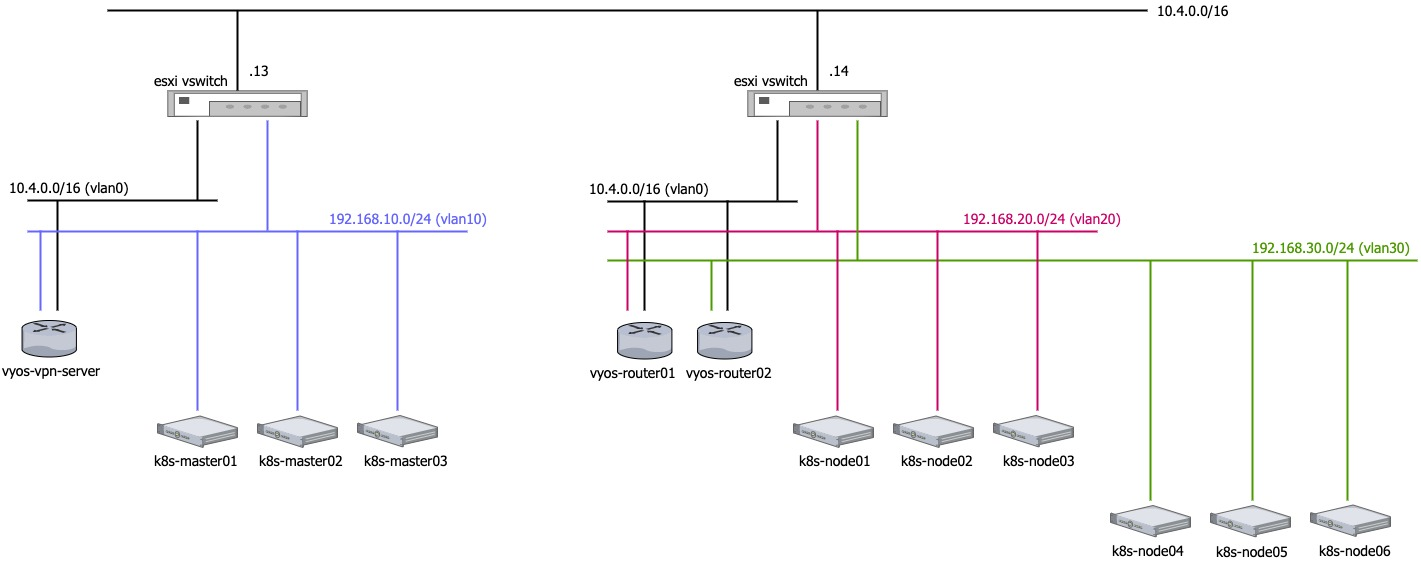
\includegraphics[width=100mm]{./figures/system-diagram.jpg}
\caption{システム構成図}
\end{center}
\end{figure}

%%% Local Variables:
%%% mode: japanese-latex
%%% TeX-master: "../bthesis"
%%% End:
